%We investigate the ability of NMT models to translate fairly% !TEX root = thesis-main.tex

\chapter{Translating Idiomatic Expressions}
\label{chapter:research-04}

\section{Introduction and research questions}

In Chapter~\ref{chapter:research-01}, we experimented with changing the scope of the context from sentence-level to document-level to capture the meaning of ambiguous words. 
In Chapters~\ref{chapter:research-02} and \ref{chapter:research-03}, we demonstrated that added context significantly help translating rare and difficult words.
The next question we are interested in is which phenomena we still \textit{fail} to capture with current approaches to using contexts.
Neural machine translation has achieved substantial improvements in translation of different linguistic phenomena over traditional rule-based and phrase-based models. 
For instance, reordering, subject-verb agreement, double-object verbs, and overlapping subcategorization are various areas where neural models successfully overcome the limitations of phrase-based models \citep{isabelle2017challenge,bentivogli-EtAl:2016:EMNLP2016}.

In this chapter, we examine which phenomena are not fully captured by current NMT models.
NMT models use both source and target sentences as contexts to generate a target word.
We are interested in cases where this scope is not sufficient for the NMT model. 
To shed light on this vulnerability of current NMT models, we ask:

\paragraph{Research Question 3:} \acl{rq:vol} 

\medskip

 \noindent We study the ability of NMT models to translate fairly complex linguistic phenomena. 
To examine this question, in this chapter, we focus on the translation of units that possibly require cues beyond the literal context, namely idiomatic expressions. 
Idioms, a category of multiword expressions, are an interesting language phenomenon where the overall meaning of the expression cannot be inferred from the meanings of its parts.
For the most part, idiom acquisition for humans requires additional resources such as explicit definitions of the expressions.  
NMT models, however, only have access to the nearby and local context of the idiomatic expression. 

To further investigate why neural translation models struggle in this area, we ask:

 
\begin{enumerate}[label=\textbf{RQ3.\arabic* },wide = 0pt, leftmargin=2em]
\setlength\itemsep{1em}
% \setcounter{enumi}{2}
\item \acl{rq:id1}

\medskip

\noindent The first challenge for learning and evaluating idiom translation is the lack of dedicated data sets.
%
In this chapter, we address this problem by creating the first large-scale data set for idiom translation. % for German$\leftrightarrow$English . 
Building a hand-crafted data set for idiom translation is costly and time-consuming.
In this chapter, we automatically build a new bilingual data set for idiom translation 
extracted from an existing general-purpose German$\leftrightarrow$English parallel corpus.
%
The first part of our data set consists of 1,500 parallel sentences where the German side contains an idiom, while the second part consists of 1,500 parallel sentences where the English side contains an idiom.
%
Additionally, we provide the corresponding training data sets for German$\rightarrow$English and English$\rightarrow$German translation where source sentences including an idiom phrase are identified. 

\end{enumerate}

\noindent We then study how this data set can aid in assessing the translation quality of idiomatic expressions, thus asking: 

\begin{enumerate}[label=\textbf{RQ3.2 },wide = 0pt, leftmargin=2em]

\item \acl{rq:id2}

\medskip

\noindent Having prepared the idiom translation training and test data, we investigate how to assess the translation quality of idiomatic expressions. 
The labels in our data are indicators of the existence of idioms in a sentence. 
We use these labels as an additional signal during training of the NMT model and examine whether this flag is sufficient in identifying a phrase as idiomatic and translating it correctly. 
Finally, we introduce several metrics to evaluate the translation quality of idiom phrases in a sentence. 

\end{enumerate}


 
\paragraph{Organization.} This chapter is organized as follows: 
In Section~\ref{idrel}, we provide an overview of existing work on idiom identification and translation. 
Next, in Section~\ref{idiomdata} we introduce our data collection procedure and details on the extracted training and test data. 
Section~\ref{idexperiments} describes the design of the experiments for translating idioms.
Section~\ref{idevalus} proposes various metrics to locally evaluate idiom translation and provides experimental results on the translation task and analyzes the performance. 
Finally, we discuss the conclusions and implications of this work in Section~\ref{idconc}. 



\section{Idiomatic expressions} \label{idrel}

Non-compositional multiword expressions, or idioms, are lexical semantic units where the meaning is often not merely a function of the meaning of its constituent parts \citep{10.2307/416483,doi:10.1093/applin/17.3.326}.

The non-compositionality characteristic of idiomatic expressions exists to different degrees in a language \citep{10.2307/416483}.
In English for example, for the idiom \textit{"spill the beans"}, the word \textit{`spill'} symbolizes \textit{`reveal'} and \textit{`beans'} symbolizes the \textit{`secrets'}. 
For the idiomatic expression \textit{"kick the bucket"}, on the other hand, no such analysis is possible.
Automatically identifying these idiomatic expressions in a sentence is challenging. 
In the following section, we discuss previous works in this area.

\subsection{Idiom identification} 

Expressions that potentially have idiomatic meanings can be recognized using various lexical association measures \citep{evert-krenn-2001-methods,evert-kermes-2003-experiments}.
However, other methods are necessary to decide whether a particular multiword expression (MWE) has an idiomatic use in a particular context.
\citet{katz-giesbrecht-2006-automatic} use distributional semantics as a model of context similarity to examine whether the local context of an MWE can distinguish its idiomatic use from its literal use.
\citet{salehi-cook-2013-predicting} use the translation of the components of the MWE in multiple languages to compute similarities between strings. This {compositionality score} illustrates the relative degree of compositionality of the MWE.
\citet{salehi-etal-2015-word} implement a similar approach but uses word embeddings to compute the compositionality score of an MWE.

 \citet{salton-etal-2016-idiom} use skip-thought vectors, sent2vec, first introduced by \citet{NIPS2015_5950} for idiom classification. 
 In this approach, they define the classes as to whether an MWE is used literally or idiomatically. 
More recently, \citet{klyueva-etal-2017-neural} propose to use an RNN that predicts the possible tags of an MWE. 
The system scored better in more `syntactic' MWEs like inherently reflexive verbs, light verb constructions, and verb-particle constructions.
However, they were not able to detect idioms with reasonable accuracy.

\subsection{Idiom translation}

Automatic translation of idiomatic phrases is a long-established problem in NLP \citep{Schenk:1986:IRM:991365.991458}.
As we illustrated in previous chapters, NMT models battle with translating rare words.
In a way, idioms are similar to this problem. 
While the occurrence of the expression might not be rare, the idiomatic meaning of the expression in a particular context is often uncommon \citep{salton-etal-2014-evaluation,isabelle2017challenge,agrawal-etal-2018-beating}. 
%
%
\begin{table}[htb!]
\centering
\small
\caption{Example of an idiomatic phrase in German and its translation. We compare the output of state-of-the-art commercial models (DeepL and GoogleNMT), as well as our trained model (based on OpenNMT). In translating a sentence containing this idiomatic phrase, we notice that none capture the idiom translation correctly. \label{examplesinc}}
\begin{tabularx}{0.8\linewidth}{p{2.7cm} X}
 \toprule
German phrase & \textit{eine wei{\ss}e Weste haben}  \\
 Literal translation & to have a white vest \\
 Idiomatic translation  &  to have clean slate  \\
	\midrule
 Sentence & Coca-Cola und Nestl{\'e} geh{\"o}ren zu den Unterzeichnern. Beide \textbf{haben} nicht gerade \textbf{eine wei{\ss}e Weste}. \\
  Reference translation & Coca Cola and Nestl{\'e} are two signatories with \textit{"spotty" track records}.\\
  \midrule
 DeepL   & Coca-Cola and Nestl{\'e} are among the signatories. Neither of them is \textbf{exactly the same}.  \\
GoogleNMT  & Coca-Cola and Nestl{\'e} are among the signatories. Both do not \textbf{have just a white vest}.  \\
OpenNMT & Coca-Cola and Nestl{\'e} are among the signatories. Both don't \textbf{have a white essence}.  \\
\bottomrule
\end{tabularx}
\end{table}
%
The challenge of translating idiomatic phrases in NMT is partly due
to the underlying complexity of identifying a phrase as idiomatic and generating its correct non-literal translation, and partly due
to the fact that idioms are rarely encountered in the standard data sets used for training NMT systems. 

As an example, in Table~\ref{examplesinc}, we provide an idiomatic expression in German and the literal and idiomatic translations in English.
We note that the literal translation of an idiom is not the correct translation; neither does it capture part of the meaning. 
To illustrate the problem of idiom translation we also provide the output of three
NMT systems for this sentence: GoogleNMT \citep{wu2016google}, DeepL\footnote{\url{www.deepl.com/translator}}, and the OpenNMT implementation \citep{2017opennmt} based on \citet{DBLP:journals/corr/BahdanauCB14} and \citet{luong:2015:EMNLP} trained on WMT17 parallel corpora. 
All systems fail to generate the proper translation of the idiomatic expression. 
This problem is particularly pronounced when the source idiom is very different from its equivalent in the target language, as is the case here.


Although there are a number of monolingual data sets available for identifying idiomatic expressions \citep{muzny2013automatic,markantonatou2017proceedings}, there is limited work on building a parallel corpus annotated with idioms, which is necessary to investigate this problem more systematically.  
\citet{salton-ross-kelleher:2014:HyTra} selected a small subset of 17 English idioms, collected 10 sentence examples for each idiom from the Internet, and manually translated them into Brazilian-Portuguese to use for translation.
\citet{isabelle2017challenge} built a challenge set of 108 short sentences that each focus on one difficult phenomenon of the language.
Their manual assessment of the eight sentences containing an idiomatic phrase showed that NMT systems struggle with the translation of these phrases.

\citet{shao-etal-2018-evaluating} introduced a new evaluation metric for detecting literal translation errors in Chinese$\rightarrow$English translation, and concluded that idiom translation remains an open problem in MT.
\citet{moussallem-etal-2018-lidioms} released a multilingual resource on idioms currently containing five languages: English, German, Italian, Portuguese, and Russian. In this work, the authors built the data set by crawling various sources and then have them manually evaluated by native speakers.

While these approaches are valuable for studying the problem of idiom translation, they each require manual efforts to identify and label idioms.
To further research in idiom translation, we still need \textit{large-scale} training and testing resources which are hard to obtain with manual labeling.  

\section{Data collection} \label{idiomdata}

In this section, we introduce our proposed data collection procedure for building a training and test set.
We focus on German$\leftrightarrow$English translation of idioms. 
This is an established language pair commonly used in machine translation literature.
Automatically identifying idiomatic phrases in a parallel corpus requires a gold standard data set annotated manually by linguists. 
We use an online dictionary containing idiomatic and colloquial phrases\footnote{\url{www.dict.cc}}, which is built manually, as our gold standard for extracting idiom phrase pairs. 

Examining the WMT German$\leftrightarrow$English test sets from 2008 to 2016 \citep{bojar-EtAl:2017:WMT1}, we observe very few sentence pairs containing an idiomatic expression. 
The standard parallel corpora available for training however contain a sizeable number of such sentence pairs.
Therefore, we automatically select sentence pairs from the training corpora where the source sentence contains an idiom phrase to build the new test set.
Note that we only focus on idioms on the source side and we have two separate lists of idioms for German and English.
Hence, we independently build two test sets (for German idiom translation and English idiom translation) with different sentence pairs selected from the parallel corpora.

 \begin{table}[htb!]
\centering
\small
\caption{Two examples displaying different constraints of matching an idiom phrase with occurrences in the sentence. \label{two}}
\begin{tabularx}{0.85\linewidth}{@{\ }l @{\ \ \ }X@{\ }}
 \toprule
German idiom & \textit{alles {\"u}ber einen kamm scheren}  \\
English equivalent & to measure everything by the same yardstick \\
Matching German sentence & Aber man kann eben nicht \textbf{alle} Inseln \textbf{\"{u}ber einen Kamm scheren}.\\
English translation &  But we cannot measure all islands by the same standards.\\ 
 \midrule
German idiom & \textit{in den kinderschuhen stecken}  \\
English equivalent & to be in the fledgling stage \\
Matching German sentence & Es \textbf{steckt} immer noch \textbf{in den Kinderschuhen}. \\
English translation &  It is still in its infancy. \\
\bottomrule
\end{tabularx}
\end{table}

Depending on the language, the words making up an idiomatic phrase are not always contiguous in a sentence. 
For instance, in German, the subject can appear between the verb and the prepositional phrase making up the idiom. 
German also allows for several re-orderings of the phrase.

In order to generalize the process of identifying idiom occurrences, we lemmatize the phrases and consider different re-orderings of the words in the phrase as an acceptable match. 
%Table~\ref{exmp} showcases an examples of this match in the corpora.
We also allow for a fixed maximum number of words to occur in between the words of an idiomatic phrase.
%In table~\ref{exmp}, the second example showcases a sentence pair matched with this constraint.
Table~\ref{two} shows two examples of idiom occurrences that match these criteria.
Following this set of rules, we extract sentence pairs containing idiomatic phrases and create a set of sentence pairs for each unique idiom phrase.


There are various ways of combining regular and idiomatic sentences and building training and test data. 
We know that the NMT model is capable of translating a word correctly at test time if it has observed it at training time.
In the previous chapters, we showed that the frequency of occurrences in the training data and the quality of the contexts are important factors in helping the model learn to translate. 
Motivated by this, we distribute sentences with idiomatic phrases between training and test sets so that there are no idioms in the test set that we have not {seen} during training.
%It is preferable if there are a sufficient number of occurrences during training. 
We also make sure that there is no overlap between the training and test sets. 

\begin{figure*}[hbt!]
\centering
%\includegraphics[width=\linewidth]{./fig/augomni222.pdf}
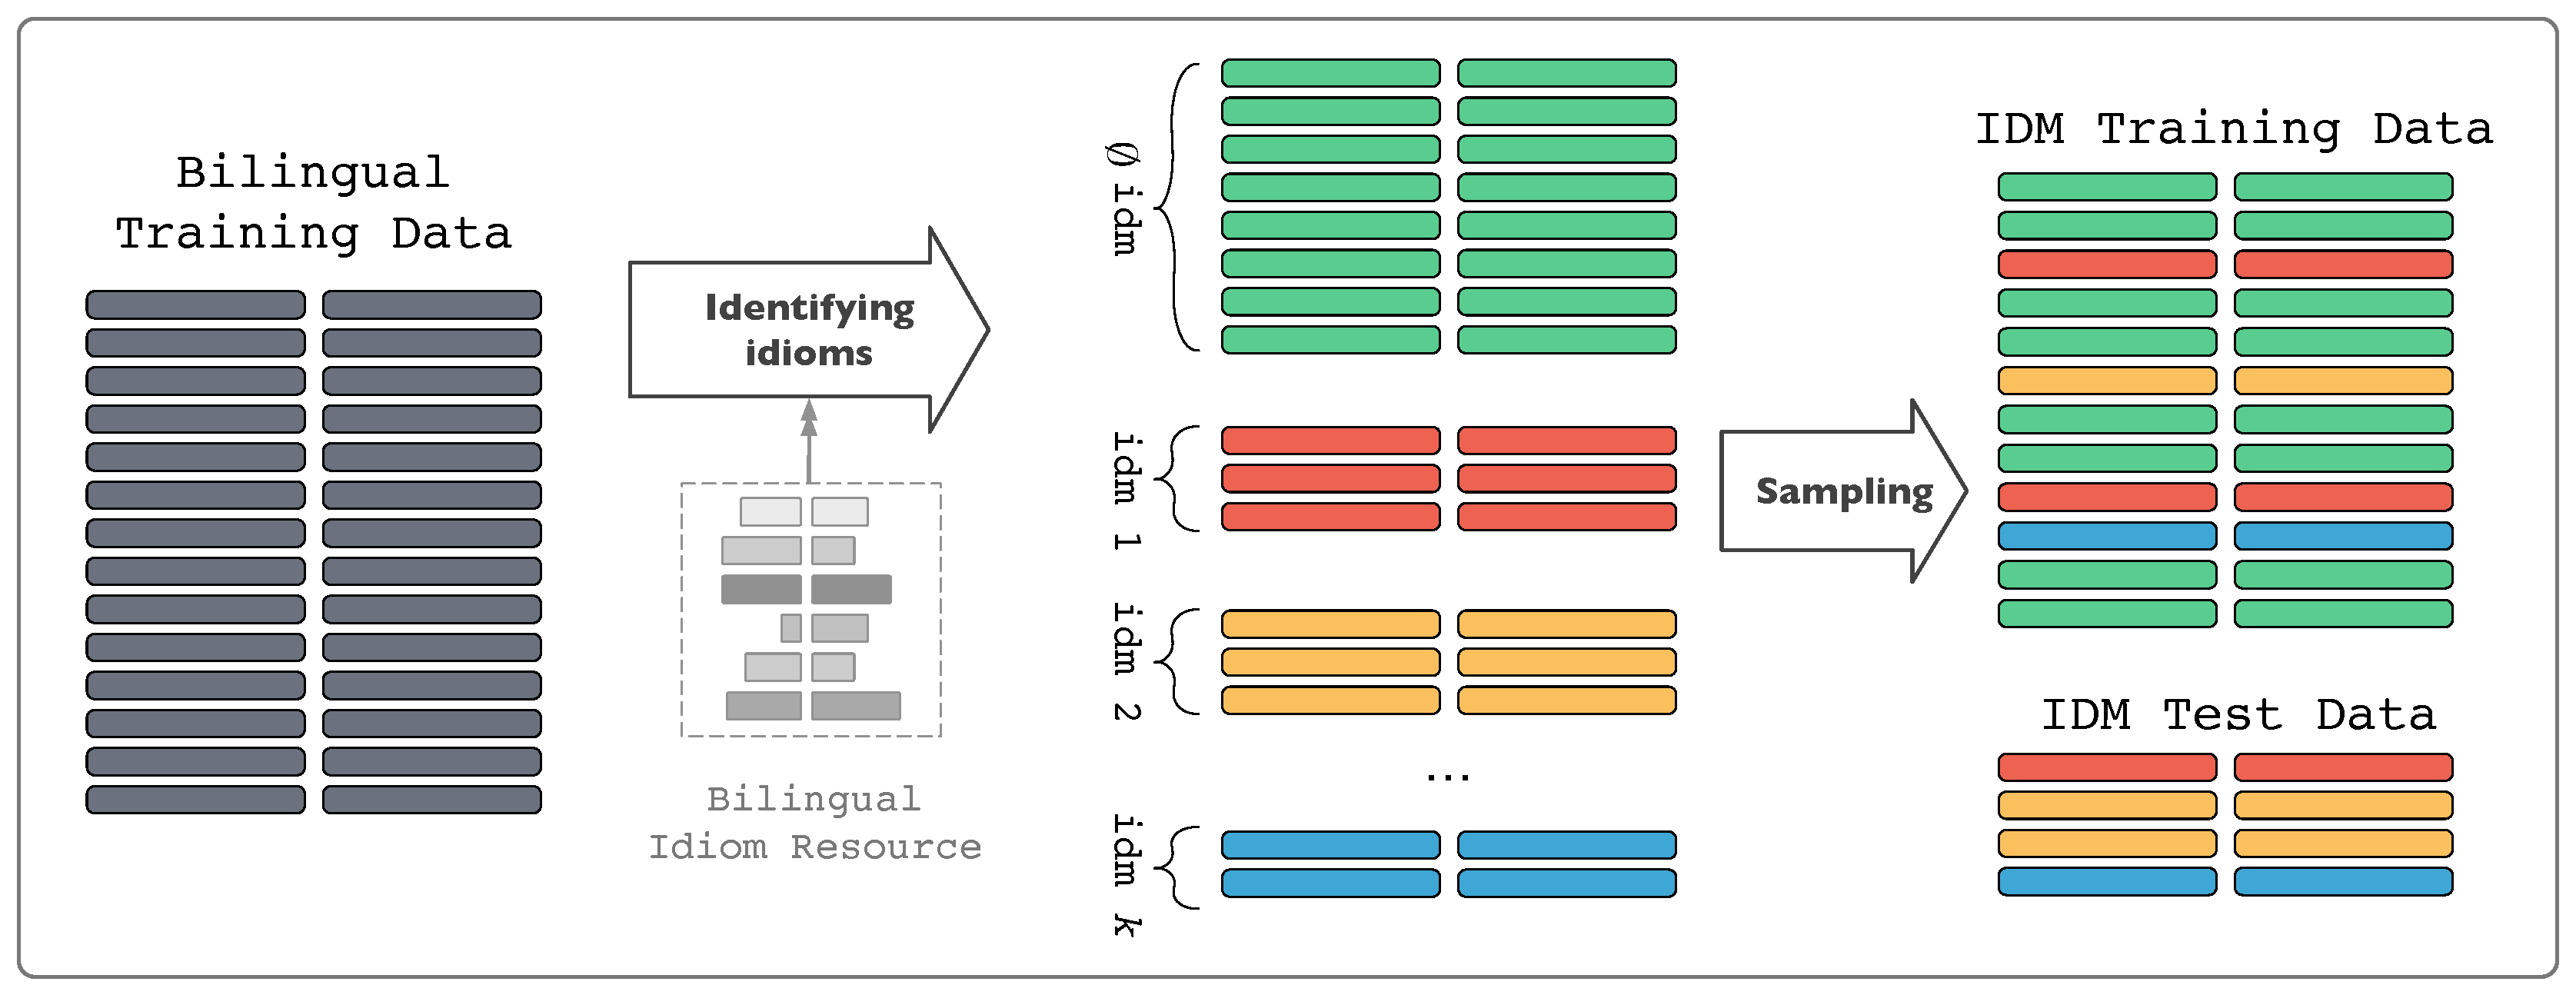
\includegraphics[width=0.95\linewidth]{06-research-04/figs/data.pdf}
\caption{The process of data collection and construction of the test set containing only sentence pairs with idiomatic phrases.}
\label{augfig2}
\end{figure*}

 \begin{table}[htb!]
\centering
\small
\caption{Statistics of the constructed German and English idiom translation data sets. %Sentence pairs are based on the training and test sets. 
\label{stats}}
\begin{tabular}{l r}
 \toprule
  German idiom translation data set & \\
  \midrule
Number of unique idioms & 103   \\
  Training size & 4.5M \\   
  Idiomatic sentences in training data & 1848 \\
 Test size & 1500  \\
\toprule
  English idiom translation data set & \\
  \midrule
Number of unique idioms &  132  \\
  Training size & 4.5M \\
  Idiomatic sentences in training data & 1998  \\
 Test size & 1500  \\
\bottomrule
\end{tabular}
\end{table}


Considering these principles, we build the training and test data as follows:
First, we sample without replacement from WMT data sets and select individual sentence pairs to build the idiom test set.
To build the new training data, we use the remaining sentence pairs in each idiom set as well as the sentence pairs from the original parallel corpora that did not include any idiomatic phrases.
In this process, we ensure that for each idiomatic expression there is at least one occurrence in both training and test data and that no sentence pair is included in both training and test data. 

  \begin{table*}[htbp]
  \rotatebox{90}{
\begin{minipage}{\textheight}
\begin{center}
% \begin{center}
 \caption{Examples from the German idiom translation test set.  \label{biggest}}
 \begin{tabularx}{0.85\linewidth}{lX}
       \toprule
       German idiom & \textit{in den kinderschuhen stecken} \\
       English equivalent &  to be in the fledgling stage   \\
       German sentence &     Eine Bemerkung, Gentoo/FreeBSD \textbf{steckt} noch \textbf{in den Kinderschuhen} und ist kein auf Sicherheit achtendes System. \\
       English sentence &     Note that Gentoo/FreeBSD is still \textbf{in its infancy} and is not a security supported platform. \\
       \midrule
       German idiom & \textit{den kreis schlie{\ss}en}   \\
       English equivalent  &  to bring sth. full circle      \\
       German sentence  & Die europ{\"a}ische Krise \textbf{schlie{\ss}t den Kreis}.\\
       English sentence  & The European crisis is \textbf{coming full circle}. \\
\midrule
       German idiom &    \textit{auf biegen und brechen} \\
       English equivalent   & by hook or crook    \\
       German sentence  & Nehmen wir zum Beispiel die W{\"a}hrungsunion: Sie soll \textbf{auf Biegen und Brechen} eingef{\"u}hrt werden.\\
       English sentence  & Take, for example, the introduction -\textbf{come what may}- of the single currency.\\
\midrule
       German idiom &  \textit{sie haben das wort} \\
       English equivalent  &   the floor is yours    \\
       German sentence  & Berichterstatterin. - (FR) Herr Pr{\"a}sident! Danke, dass \textbf{Sie} mir \textbf{das Wort} erteilt \textbf{haben}.\\
       English sentence  & rapporteur. - (FR) Mr President, thank you for \textbf{giving} me \textbf{the floor}.\\
\bottomrule
 \end{tabularx}
 \end{center}
\end{minipage}
}
 %\end{center}
 \end{table*}
 
Figure~\ref{augfig2} visualizes the process of constructing the new training and test sets.
As a result of this construction, for each language direction, we obtain a targeted test set for idiom translation and the corresponding training corpus representing a natural distribution of sentences with and without idioms.
We annotate each sentence pair with the canonical form of its source-side idiom phrase and its equivalent in the target language. 

Table~\ref{stats} provides some statistics of the two data sets. 
For each unique idiom in the test set, we also provide the frequency of the respective idiom in the training data. 
Note that this is based on the lemmatized idiom phrase under the constraints mentioned in Section~\ref{idiomdata} and is not necessarily an exact match of the phrase.
Table~\ref{biggest} shows several examples from the data set for German idiom translation. 
We observe that for some idioms the literal translation in the target language is close to the actual meaning, while for others it is not the case.

Note that multiword expressions that at times have an idiomatic meaning can also be translated literally depending on the context (e.g., \textit{"spill the beans"} to literally describe the act of \textit{spilling the beans}). 
This data set represents this additional difficulty: Models cannot just memorize fixed translation of idioms but also have to consider the specific context in which they are used.

\section{Translation experiments} \label{idexperiments}
    
While the main focus of this chapter is to generate data sets for training and evaluating idiom translation, we also perform a few NMT experiments using our data set to measure the problem of idiom translation on large-scale data. 

In the first experiment, following the conventional settings, we do not use any labels indicating whether a particular phrase is used idiomatically or not in the training data.
In the second experiment, we use the labels in the training data as an additional feature to investigate the effect of informing the model of the existence of an idiomatic phrase in a sentence during training.
We perform %two 
a German$\rightarrow$English experiment by providing the model with additional input flags.
This approached is similar to the work by \citet{sennrich-etal-2016-controlling}, where they control the honorifics produced at test time by adding a side constraint to the source side. 

The additional flag indicates whether a source sentence contains an idiom
and are implemented as a special extra token \texttt{<idm>} that is prepended to each source sentence containing an idiom both in the training and test data.
This a simple approach that can be applied to any sequence-to-sequence architecture. 

%Most NMT systems have a sequence-to-sequence architecture where an encoder builds up a representation of the source sentence and a decoder, using the previous LSTM hidden states and an attention mechanism, generates the target translation \citep{DBLP:journals/corr/BahdanauCB14,sutskever2014sequence,cho2014properties}.
We use a 4-layer attention-based encoder-decoder model as described in Section~\ref{RNN} trained with hidden dimension size of 1000, and batch size of 80 for 20 epochs. 
%
In all experiments, the NMT vocabulary is limited to the most common 30K words in both languages and we preprocess source and target language data with Byte Pair Encoding (BPE) \citep{sennrich-haddow-birch:2016:P16-12} using 30K merge operations. 
We also use a phrase-based translation system similar to Moses \citep{koehn-etal-2007-moses} as baseline to measure PBMT performance for idiom translation.
Several examples of our idiom translation test set and the output translations of the PBMT and NMT models are illustrated in Table~\ref{smtnmt}.

  \begin{table*}[htbp]
%  \rotatebox{90}{
%\begin{minipage}{\textheight}
\begin{center}
% \begin{center}
 \caption{Examples from the resulting test set of sentence pairs containing idiomatic expressions. NMT and PBMT translations of sentences are provided, highlighting the challenge of idiom translation.  \label{smtnmt}}
 \begin{tabularx}{0.95\linewidth}{lX}
       \toprule
%       \textsc{src} & Alles, was ich brauche, finde ich \textbf{vor Ort}. \\
   %    \textsc{ref} & I can find everything I need \textbf{locally}. \\
      % PBMT  & everything I do, I think, \underline{on the ground}. \\
       %NMT  &  All I need is \underline{on site}. \\
       %\midrule
 \textsc{src} &   Seitdem aber begannen sich zwischen Pol\'{i}vka und Harabi\v{s} die Streitigkeiten zu h\"{a}ufen, die in der Absetzung ``K\"{o}nig Boleslavs I. gew\"{a}hlt \textbf{bis zum Sankt-Nimmerleins-Tag}'' gipfelten. \\
       \textsc{ref} &  From then on , quarrels begin to accumulate between Pol\'{i}vka and Harabi\v{s} , which culminated in the dethronement of ``the king Boleslav I elected \textbf{forever and ever}''.   \\
       PBMT  &  Since then, however, the disputes between Pol\'{i}vka and Harabi\v{s} began to accumulate, culminating in the departure of King Boleslavs I.   \\
       NMT  &   Since then, but began between Pol\'{i}vka and Harabi\v{s} disputes to accumulate in the removal ``king Boleslavs I. elected by the \underline{Sankt-Nimmerleins-Tag} culminated''.    \\
              \midrule
 \textsc{src} &   Sie wurde \textbf{vor Ort} not\"{a}rztlich behandelt und von Rettungskr\"{a}ften in ein Krankenhaus gebracht. \\
       \textsc{ref} &   She was treated \textbf{at the site} by an emergency doctor and taken to hospital by ambulance.  \\
       PBMT  &  It was treated \underline{on site in the field}, and it was brought to a hospital from the rescue forces.   \\
       NMT  &   she was \underline{on the ground} and not\"{a}rztlich treated by rescue workers in a hospital.    \\
              \midrule
 \textsc{src} & Janson ist selbst ein \textbf{alter Hase} in seinem Metier, der Schauspielkunst.   \\
       \textsc{ref} &   Janson is an \textbf{old hand} himself when it comes to his profession, the art of acting.  \\
       PBMT  &   Janon himself is an \underline{old hase} in his painter, the artistic art.  \\
       NMT  &    Janson itself is an \underline{old hand} in his subjects, the schauspielkunst.   \\
       \midrule
     \textsc{src} &   Mit unserer Mitteilung vom letzten Sommer haben wir \textbf{den Stein ins Rollen} gebracht und demonstriert, dass Europa an der Erarbeitung eines internationalen Instruments beteiligt ist. \\
       \textsc{ref} & Our communication of last summer enabled us to \textbf{get things up and running} and to demonstrate that Europe was participating in the drawing up of an international instrument. \\
       PBMT  &    With our communication of last summer we \underline{have the ball rolling} and demonstrated that Europe in the drafting of an international instrument is involved. \\
       NMT  &   With our communication last summer, we \underline{launched the stone} and demonstrated that Europe is involved in the development of an international instrument. \\
\bottomrule
 \end{tabularx}
 \end{center}
 \end{table*}
 
\section{Idiom translation evaluation} \label{idevalus}

Ideally, idiom translation should be evaluated manually, but this is a very costly process.
%one should do manual evaluation of idiom translations, however since it is costly, in this work we consider using automatic metrics. 
Automatic metrics, on the other hand, can be used on large data sets at no cost and have the advantage of replicability (Section~\ref{bgexp}).
We use three metrics to evaluate the translation quality with a specific focus on idiom translation accuracy: BLEU, Modified Unigram Precision, and Word-level Idiom Accuracy. We describe each metric below.

\subsection{BLEU} The traditional BLEU score \citep{Papineni2001}, discussed in Section~\ref{bgexp}, is a good measure to determine the overall quality of the translations. 
However, this measure considers the precision of \textit{all} $n$-grams  in a sentence and by itself does not focus on the translation quality of the idiomatic expressions.

\subsection{Modified unigram precision} 
To specifically concentrate on the quality of the translation of idiomatic expressions, we also look at the \textit{localized} precision. 
In this approach, we translate the idiomatic expression in the context of a sentence and only evaluate the translation quality of the idiom phrase. 

To isolate the idiom translation in the sentence, we look at the word-level alignments between the idiomatic expression in the source sentence and the generated translation in the target sentence. 
We use \texttt{fast-align} \citep{dyer-chahuneau-smith:2013:NAACL-HLT} to extract word alignments.
Since idiomatic phrases and the respective translations are not contiguous in many cases, we only compare the unigrams of the two phrases.
We compute unigram matches between the reference translation and the translation output, the $candidates$ set, as follows:
\begin{equation} 
UniPrec = \frac{ \sum\limits_{\vt{C} \in \{Candidates\}}^{} \sum\limits_{{\unigram} \in \vt{C}}^{} \countop_{clip}({\unigram}) }{  \sum\limits_{\vt{C'} \in \{candidates\}}^{} \sum\limits_{{\unigram }' \in \vt{C'}}^{} \countop({\unigram}')  }
\end{equation}

\noindent where $\countop_{clip} = \min(\countop, \textit{max\_ref\_count})$.
By computing the clipped count, we truncate each word's count so that it does not exceed the largest count observed in a reference for that word.
Note that for this metric %and \textit{Word-level Idiom Accuracy} 
we have two references: The idiom translation as an independent expression, and the human-generated idiom translation in the target sentence. 

\subsection{Word-Level idiom accuracy} We also use another metric to evaluate the word-level translation accuracy of the idiom phrase. 
We use word alignments between source and target sentences to determine the number of correctly translated words.
We use the following equation to compute the accuracy:
\begin{align} 
WAcc = \frac{H-I}{N}
\end{align} 

\noindent where $H$ is the number of correctly translated words, $I$ is the number of extra words in the idiom translation, and $N$ is the number of words in the gold idiomatic expression.

\smallskip

\begin{table*}[htb!]
\begin{center}
\caption{Translation performance on the German idiom translation test set. \textit{Word-level Idiom Accuracy} and \textit{Unigram Precision} are computed only on the idiom phrase and its corresponding translation in the sentence.   \label{numbers}}
\begin{tabularx}{0.72\textwidth}{@{\extracolsep{4pt}} l cccc}
\toprule
 & \multicolumn{1}{c}{\bf WMT08-16}  & \multicolumn{3}{c}{\bf Idiom test set}\\ \cline{2-2} \cline{3-5}
    \bf Model &  BLEU  &   BLEU  &    UniPrec &  WAcc  \\ 
     \toprule
PBMT baseline & 20.2  & 19.7  &  57.7 & 71.6 \\
NMT baseline   &  26.9  &    24.8       &  53.2 &   67.8  \\
NMT  \textsc{src} flag  & 25.2  &  22.5       & 64.1 & 73.2     \\
NMT \textsc{tgt} flag  & 17.8  & 16.2           &   54.3 &  64.0  \\
      \bottomrule
\end{tabularx}
 \end{center}
\end{table*}

\subsection{Evaluation results}
Table~\ref{numbers} presents the results for the translation task using different metrics. 
Looking at the overall BLEU scores, we observe that baseline performance on the idiom-specific test set is lower than on the union of the standard test sets (WMT 2008-2016). 
While the scores on these two data sets are not directly comparable, this result is in line with previous findings that sentences containing idiomatic expressions are harder to translate \citep{isabelle2017challenge}.
We can also see that the performance gap is %However, this is 
not as pronounced for a PBMT system, suggesting that phrase-based models are capable of \textit{memorizing} the idiomatic phrases to some extent.

The NMT model using a special input flag to indicate the presence of an idiom in the source sentence performs better than PBMT but slightly worse than the NMT baseline in terms of BLEU.
Despite this drop in BLEU performance, by examining the \textit{unigram precision} and \textit{word-level idiom accuracy} scores, we observe that this model generates more accurate idiom translations.
When comparing this to having the idiom flag on the source or target side, we observe a significant difference:
The experiment with the target flag performs the worst, partially because during inference, only the source sentence is available and hence there is no contextual signal to aid the model.
 
 \begin{figure*}[ht!]
\centering
\begin{subfigure}[h]{0.495\textwidth}
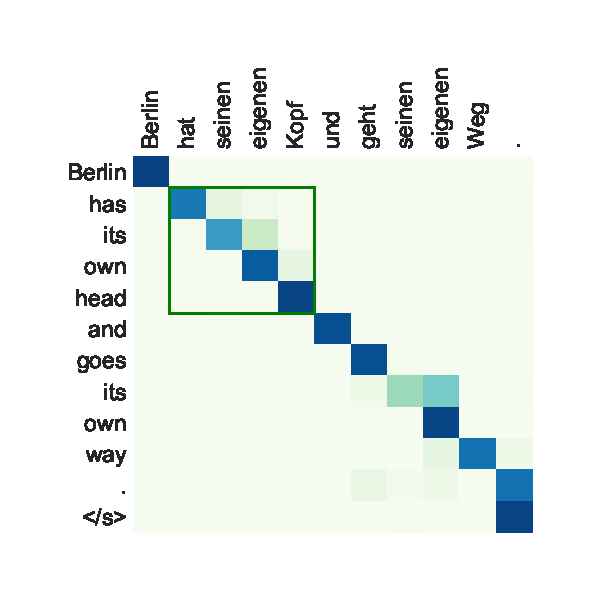
\includegraphics[width=\linewidth]{06-research-04/figs/idiomexam2.pdf}
\end{subfigure}
\begin{subfigure}[h]{0.495\textwidth}
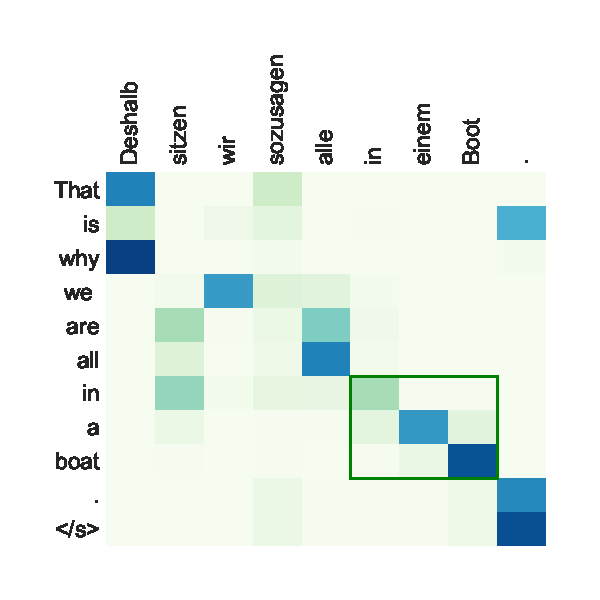
\includegraphics[width=\linewidth]{06-research-04/figs/idiomexam3.pdf}
%\caption{Attention matrix for translation of a German sentence. The blocked area marks the idiomatic expression and its generated translation. The reference translation is: \textit{``x''}\label{att2}}
\end{subfigure}
\caption{Attention visualization of the translation of two sampled German sentences. Darker color means higher weight. The blocked area marks the idiomatic expression and its generated translation. The reference translations are: (left) \textit{``Berlin \underline{has a mind of its own} and is doing its own thing.''} and (right) \textit{``We are therefore all \underline{in the same boat}, so to speak.''} \label{att2}}
\end{figure*}


Figure~\ref{att2} illustrates the attention distribution of the NMT model during translation of an example German sentence. 
We expected that in order to translate each word in the idiomatic expression correctly, the model would pay a noticeable degree of attention to the other words in the expression. 
However, we see that it does not happen and the model essentially translates the sentence word by word, i.e., literally. 
%We suspect that for idiom translation to be successful, NMT models need a stronger signal from context.
%
These preliminary experiments reiterate the problem of idiom translation with neural models, and in addition show that with a labeled data set, we can devise simple models to address this problem to some extent.


\section{Conclusion} \label{idconc}


Motivated by our observations in Chapters~\ref{chapter:research-02} and \ref{chapter:research-03} that illustrate the importance of local context on learning difficult words, we further explored in this chapter some shortcomings of current models.
Concretely, we were interested in finding cases where NMT models are unsuccessful.
One case of a complex language phenomenon is idiom translation where it is very difficult to infer the meaning of the phrase without explanation and only from the observed context.

To investigate the behaviour of NMT models in translating idiomatic expressions, we asked:

 
\begin{enumerate}[label=\textbf{RQ3.\arabic* },wide = 0pt, leftmargin=2em]
\setlength\itemsep{1em}
\item \acl{rq:id1}

\medskip

\noindent We identified two main challenges when translating idiom phrases, namely lack of dedicated data sets and lack of targeted evaluation metrics.
%As an essential step towards assessing idiom translation quality in neural models, we require an explicitly tailored test data.
To address this problem, we have extracted a parallel data set for training and testing idiom translation for German$\rightarrow$English and English$\rightarrow$German.
%
In the test sets, we included sentences with at least one idiom on the source side.
In the training set, we included a mixture of idiomatic and non-idiomatic sentences with labels to distinguish between the two.
We release our new data sets which can be used to further investigate and improve NMT performance of idiom translation.
Using our new resources, we performed preliminary translation experiments to evaluate the quality of idiom translation.
Experiments on this test set showed PBMT models scored higher than NMT models on our metrics which explicitly measure idiom translation quality. 

\item \acl{rq:id2}

\medskip

\noindent We observed that even though the NMT model achieved a higher overall BLEU score, it performed worse on idiom translation metrics in comparison with PBMT model.
%This is in agreement with previous work on investigating the weak points of neural models.
Next, we studied whether a flag in the training data can help to distinguish between when a phrase is to be translated literally and when it should be translated idiomatically.
Our experiments showed that adding a side flag during training improves the quality of idiom translation.
However, we found that the BLEU score on standard test sets declined.
Our experiments suggest that there is no correlation between overall BLEU scores and the localized precision of idiomatic phrase translations.

%

\end{enumerate}

 \noindent It allows us to return to our more general research question:

\paragraph{Research Question 3:} \acl{rq:vol} 

\medskip

 \noindent To answer this question, we specifically examined non-compositional multiword expressions.
%Idiom translation is one of the more difficult challenges of machine translation. 
Since the literal meaning of the components is different from the idiomatic meaning of the entire expression, the model needs to know in which context to translate it literally and in which idiomatically. 
We showed that NMT models perform poorly on idiom translation despite their overall strong advantage over previous MT paradigms. 
We conclude that further research on idiom translation can benefit from having a dedicated data set. 

\noindent In the next chapter, we continue investigating this question by examining cases where there are no complex linguistic phenomena, such as non-compositional phrases, in the observed context.









